% Created 2021-04-15 Thu 18:00
% Intended LaTeX compiler: pdflatex
\documentclass[12pt]{report}
\usepackage[utf8]{inputenc}
\usepackage[T1]{fontenc}
\usepackage{graphicx}
\usepackage{grffile}
\usepackage{longtable}
\usepackage{wrapfig}
\usepackage{rotating}
\usepackage[normalem]{ulem}
\usepackage{amsmath}
\usepackage{textcomp}
\usepackage{amssymb}
\usepackage{capt-of}
\usepackage{hyperref}
\usepackage{minted}
\usepackage[]{minted}
\usepackage{tcolorbox}
\usepackage{etoolbox}
\def\mytitle{??? Program Code ???}
\BeforeBeginEnvironment{minted}{\begin{tcolorbox}[title=\hfill \mytitle]}%
\AfterEndEnvironment{minted}{\end{tcolorbox}}%
\usepackage{hyperref}
\usepackage{algorithmic}
\usepackage{pdfpages}
\makeatletter
\AtBeginEnvironment{minted}{\dontdofcolorbox}
\def\dontdofcolorbox{\renewcommand\fcolorbox[4][]{##4}}
\makeatother
\usepackage[hmargin=25mm,vmargin=25mm]{geometry}
\setlength{\parskip}{1em}
\setlength{\parskip}{1em}
\usepackage[backend=biber,style=alphabetic]{biblatex}
\addbibresource{References.bib}
\usepackage{MyUnicodeSymbols}
\usepackage[dvipsnames]{xcolor} % named colours
\usepackage{color}
\definecolor{darkred}{rgb}{0.3, 0.0, 0.0}
\definecolor{darkgreen}{rgb}{0.0, 0.3, 0.1}
\definecolor{darkblue}{rgb}{0.0, 0.1, 0.3}
\definecolor{darkorange}{rgb}{1.0, 0.55, 0.0}
\definecolor{sienna}{rgb}{0.53, 0.18, 0.09}
\hypersetup{colorlinks,linkcolor=darkblue,citecolor=darkblue,urlcolor=darkgreen}
\setcounter{secnumdepth}{0}
\author{Curtis D'Alves}
\date{April 15, 2021}
\title{Teaching Portfolio}
\hypersetup{
 pdfauthor={Curtis D'Alves},
 pdftitle={Teaching Portfolio},
 pdfkeywords={},
 pdfsubject={},
 pdfcreator={Emacs 27.1 (Org mode 9.4.4)}, 
 pdflang={English}}
\begin{document}



\setminted[haskell]{fontsize=\footnotesize}
\setminted[agda]{fontsize=\footnotesize}
\def\labelitemi{$\diamond$}
\def\labelitemii{$\circ$}
\def\labelitemiii{$\star$}

% Level 0                 Level 0
% + Level 1               ⋄ Level 1
%   - Level 2       --->      ∘ Level 2
%     * Level 3                   ⋆ Level 3
%

\begin{center}


\thispagestyle{empty}

{\color{white}{.}}

\vspace{5em}

{\Huge Professional Teaching Portfolio Of}

\vspace{1em}

{\Large \href{mailto:curtis.dalves@gmail.com}{Curtis D'Alves}}

\vspace{2em}
Ph.D Candidate and Sessional Instructor

Department of Computing and Software

McMaster University

\vspace{2em}
Last Edited: \today

\vfill

\def\mytitle{{\sc Contact \hspace{12em} \color{grey}{.} }}
\begin{minted}[]{haskell}
Email:                                                        curtis.dalves@gmail.com
Phone:                                                        +905-870-3907
\end{minted}
\end{center}

\thispagestyle{empty}
\tableofcontents
\newpage

\part{Teaching Philosophy}
\label{sec:orgbf2f24d}
\section{My core personal beliefs on teaching}
\label{sec:org3901377}

\textbf{Teaching is a responsibility}. When a person assumes the role of teacher,
they take on the responsibility of guiding a learners experience. On the other
hand, the learner must yield a certain degree of trust with the teacher. This
is not to say a students learning experience solely relies on a teacher, but
it is necessary to recognize this dynamic to effectively understand the role.
It is a teachers responsibility to never betray the trust of a student, this
responsibility is multi-faceted and vast but put broadly the teacher must
always put the students well being first and foremost. This means results
achieved by conventional means of assessment cannot be the teachers only
priority.

\noindent
\textbf{Good teaching challenges and inspires students}. A teacher should offer the
students more than what can be offered through a textbook or pre-recorded
lectures. A teacher should present students with challenges to overcome, and
inspire them to want to do so of their own volition. I entered university with
a singular goal, acquire a degree. However during my first year of university,
I met a professor that I'd come to do a student research project with during
the summer that would change my outlook on education. He presented me with an
opportunity to do real research, and although I was highly under-qualified at
the time he set up series of challenges/stepping stones that allowed me to
work up to the level of competence necessary to be useful. I wish to inspire
other students the way he inspired me.

\noindent
\textbf{Teaching should be accessible}. Everyone should have access to education, and
teachers should be aware and accommodating of different accessibility issues
that their students may face. Teachers are often to quick to assume their
methods of assessment or presentation are the only reasonably effective way to
teach, and that it is the responsibility of the student to adapt to them no matter
their circumstances. This loses sight of the true goals of teaching, to give
students the skills and knowledge they need to succeed.

\section{My teaching strategies}
\label{sec:orgdae85cd}

\textbf{I employ Active Learning methods in my lectures and teaching material}.
Active learning makes use of various activities to break up the otherwise
passive experience of learning in traditional lectures. It puts a higher
degree of responsibility on the student, challenging them during the learning
process. And there is possibly no more appropriate field to employ active
learning then computing and software. Interfacing with a computer allows a
level of live assessment not achievable otherwise. By interspersing lecture
content with live coding activities and discussion sessions students have a
much deeper level of engagement with the material, and receive a much more
adequate level of feedback than conventional assessment methods. Regular
lecture sessions cease to be a passive experience where students show up
simply to listen to a professor present a topic and become a challenge for
learners to overcome.

\noindent
\textbf{I provide real world applications of concepts being taught wherever
possible}. Most students in STEM come to university with the dream of one day
acquiring the skills to build something truly useful. For these students, the
traditional university experience can be extremely disheartening. Whole
subjects (calculus for example) can seem like nothing more than a form of
academic hazing, meant to give students a hard time rather than provide them
with useful skills. This is not to say STEM students shouldn't be taught
calculus, but that if done in a way that doesn't reflect it's applicability
it can be a hindrance to their academic development. 

\noindent
\textbf{I design my course content following Universal Design for Learning
principles}. When appropriate, I provide course content in as many different
means of representation as reasonable. This means implementing redundancies
for visual and audio representation in lectures and video presentations, which
can be as simple as making sure to fully explain slide content verbally and
providing all verbally explained content in slides and text documents. I also
encourage note sharing (either for bonus marks or a means of assessment with
exemptions) to help students who have difficulty taking notes. Another
principle of Universal Design for Learning I follow is providing students with
multiple means of engaging with me. Although I encourage students to engage
with me directly in class or during office hours, I understand in person
experience can be anxiety inducing. I find online interfaces (like forums and
instant messaging / video conferencing) can be very effective alternatives for
these students.

\section{My goals as a teacher}
\label{sec:org1091e9c}

Although my teaching experience is limited, I already greatly value the
positive impacts I've had on my students. Of all the feedback I've received,
the most dear to me are from students from a different program who have stated
they were inspired by me to transfer into a computing program. The most
obvious goal any institutional teacher should have is for their students to
finish with a sufficient understanding of the course material. This is a very
valid goal and one I hold, however I don't limit myself there. My more
ambitious goal is to inspire students to want to continue learning. But this
isn't the only ambitious goal I have. I wish to not just acknowledge my
positive feedback but critically engage with and improve from my negative
feedback. The most common theme in my negative feedback (particularly from the
first few sessional positions I taught) revolve around having too high
expectations on students. I believe this stems partly from my desire to
challenge students, but also a personality flaw of lack of patience. One of
the greatest things about being a teacher is it challenges you to grow as a
person. I have seen myself become a more patient and understanding person each
year I teach not just through my interactions with students and course
feedback, but also in my personal life. It is my greatest goal that as I
continue to improve as a teacher, I continue to improve as a person.

\part{Teaching Practice}
\label{sec:orgcb011a6}
To practically apply my teaching philosophy, I continually strive to better
integrate my teaching strategies (using real-world applications, active
learning and Universal Design for Learning) in all of my course content. This
includes how I develop/present my lectures, how I develop my assessments and
what types of assessments and course materials I focus on. When I taught my
first sessional position, an experiential learning based course in the second
semester of the first year in a CS program (known as CS 1XA3), I laid out a
clear road map with an end goal of developing a Django stack (Javascript -
Python - Django - MySQL) web app managed under a GitHub repository that they
could showcase as part of their personal portfolio. I found that as long as I
could relate the concepts I was teaching as part of this end goal students
were far more inspired to engage with the content.

When I was a teaching assistant for another intro CS course (known as CS
1JC3), I assisted a professor in a series of lecture sessions he referred to
as "Discussion Sessions". In one of the three lecture sessions a week, we
would hold a lecture session that focused on calling on students and asking
them questions about the topics discussed in the previous lecture sessions
that week. The questions were designed to be high-level and divergent so they
engaged the students far more than questions with simple right or wrong
answers. When I eventually "inherited" the course as a sessional instructor, I
continued this practice as the students always seemed to remark on their value
in the year end evaluations. In the proceeding year when I taught the course
online during the 2020 pandemic, I changed things up a bit by making every
lecture section a "Discussion Session", interleaving presenting lecture
content and questions. Although this cut down the amount of content I could
cover this proved to be a worthy trade-off, actively engaging students in
content that they would demonstrate they better retained come exam time. 

In both courses I've taught as a sessional instructor, I've come to find a
focus on project based assessment to be more effective than exams. This is not
to say I didn't administer an exam, but I was open to allowing students to
shift more weight of their final mark onto projects that could be better
tailored to suit their learning needs. Although exams have their place they
are often more limited in their ability to fully assess a students
capabilities/knowledge, and often disadvantage students who have accessibility
issues making it difficult to complete assessments with short time
constraints. In general I try to be as accomadating as reasonable when finding
the correct method of assessment for an individual student. Another example of
this is the Discussion Sessions I mentioned in CS 1JC3, although I found these
sessions to be very valuable for the majority of the class, some students with
anxiety issues found answering questions on the spot in front of a class an
in-due burden. For these students I offered alternatives such as writing up
and sharing notes taken during the lecture. When teaching you encounter a
large variety of students with different needs, and it's important to be
flexible and consult students who struggle on a individual basis to find the
correct methods to accommodate them.


\part{Teaching Experience}
\label{sec:orga4f4326}
\section{Teaching Assistantships}
\label{sec:org4fe2b1a}
\subsection{Teaching Assistant CS 1MA3}
\label{sec:orge7eee52}
\begin{itemize}
\item \textbf{Sept-Dec 2011/2012}
\item \textbf{McMaster University}
\item Instructed course tutorials and assisted in developing tutorial content and
slides. Marked assignments, midterms and exams.
\end{itemize}

\subsection{Teaching Assistant CS 1JC3}
\label{sec:org65e588b}
\begin{itemize}
\item \textbf{Sept-Dec 2013/2014/2017/2018}
\item \textbf{McMaster University}
\item Developed and lead tutorial content for
introductory Haskell and Elm and
assisted marking assignments and midterm tests.
\end{itemize}

\subsection{Teaching Assistant CS/SE 4F03}
\label{sec:orgd4df4ac}
\begin{itemize}
\item \textbf{Feb-May 2015}
\item \textbf{McMaster University}
\item Lead tutorials and taught content
pertaining to parallel programming with MPI and OpenMP in C/C++ and
marked assignments.
\end{itemize}

\subsection{Teaching Assistant CS 3EA3}
\label{sec:org29d9c4a}
\begin{itemize}
\item \textbf{Feb-May 2017}
\item \textbf{McMaster University}
\item Lead tutorials and taught content pertaining to formal methods and automated
verification of C programs in Frama-C
\end{itemize}

\section{Sessional Instructor Positions}
\label{sec:org8984049}
\subsection{Sessional Position CS 1XA3}
\label{sec:orga6bfb36}
\begin{itemize}
\item \textbf{Feb-May 2018/2019/2020}
\item \textbf{McMaster University}
\item Developed entirely original course content for lectures, labs, projects,
exams and taught all lectures and labs. The course focused around 3 projects
and taught version control with Git, Bash scripting, Web App development, and
developing a parser and simple interpreter.
\end{itemize}

\subsection{Sessional Position CS 1JC3 C02}
\label{sec:orga4c5816}
\begin{itemize}
\item \textbf{Sep-Dec 2019/2020}
\item \textbf{McMaster University}
\item Taught to Non-Computer Science students. Lead lectures and developed new
assignment content and midterms.
\end{itemize}

\part{Evidence of the Effects of Teaching}
\label{sec:org922a7eb}
\section{Teaching Evaluations}
\label{sec:orgbe5185e}
\subsection{CS 1XA3 Winter 2019 (Combined C01/C02 Sections)}
\label{sec:orgbf51254}
\textbf{Overall for this course, what is your opinion of the effectiveness of the
instructor?} (Scale: 1 Very Poor to 10 Excellent)

\begin{center}
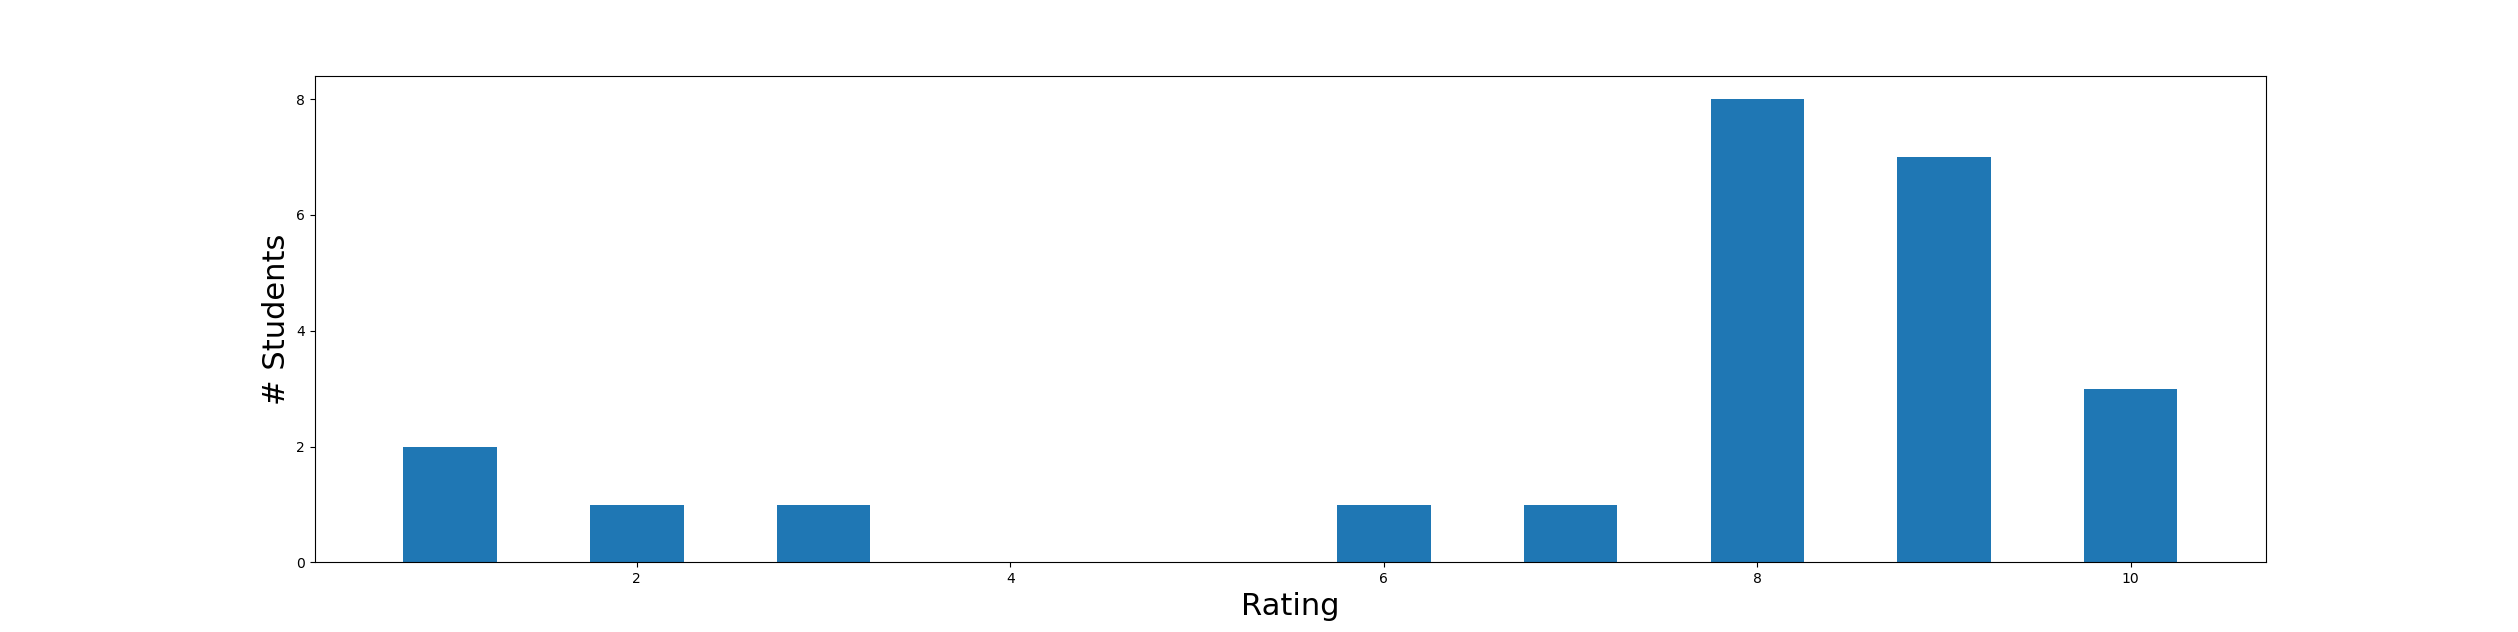
\includegraphics[width=1.0\textwidth,height=0.5\textwidth]{./course-evals/Eval_1XA3_2019_Overall.png}
\end{center}

\noindent
\textbf{Independent critical judgement was encouraged} (Scale: 1 Very Poor to 5 Excellent)

\begin{center}
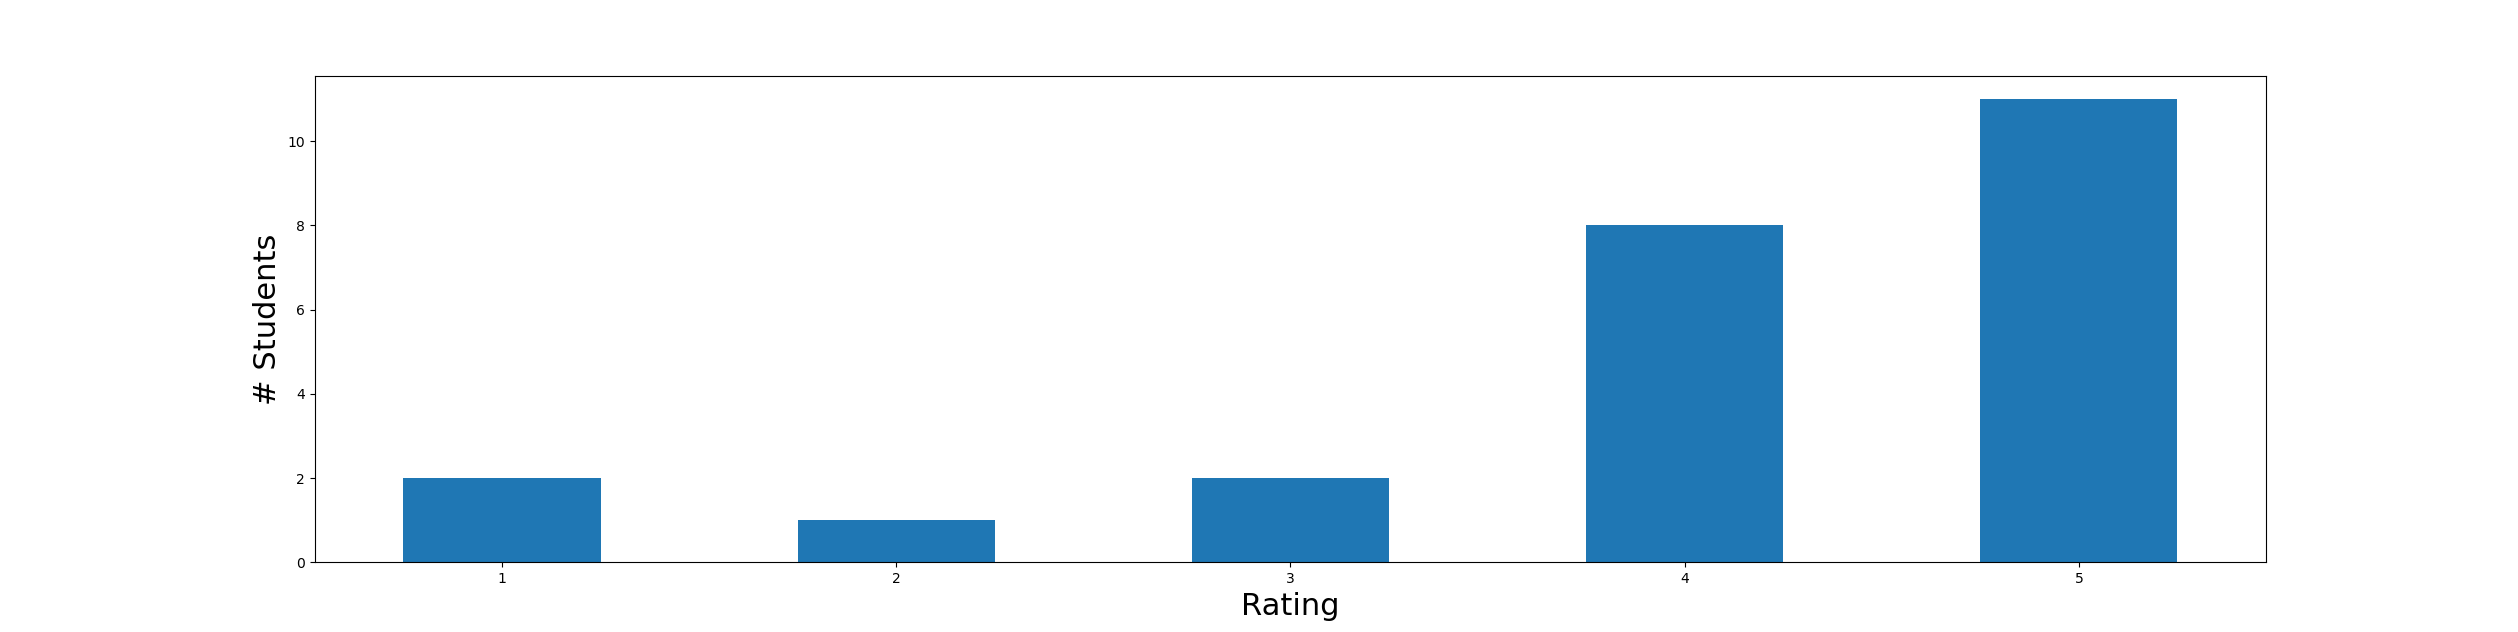
\includegraphics[width=1.0\textwidth,height=0.5\textwidth]{./course-evals/Eval_1XA3_2019_Critical.png}
\end{center}

\newpage
\noindent
\textbf{The instructor's response to students (Approachability, attitude,
availability, well-explained answers)} (Scale: 1 Very Poor to 5 Excellent)

\begin{center}
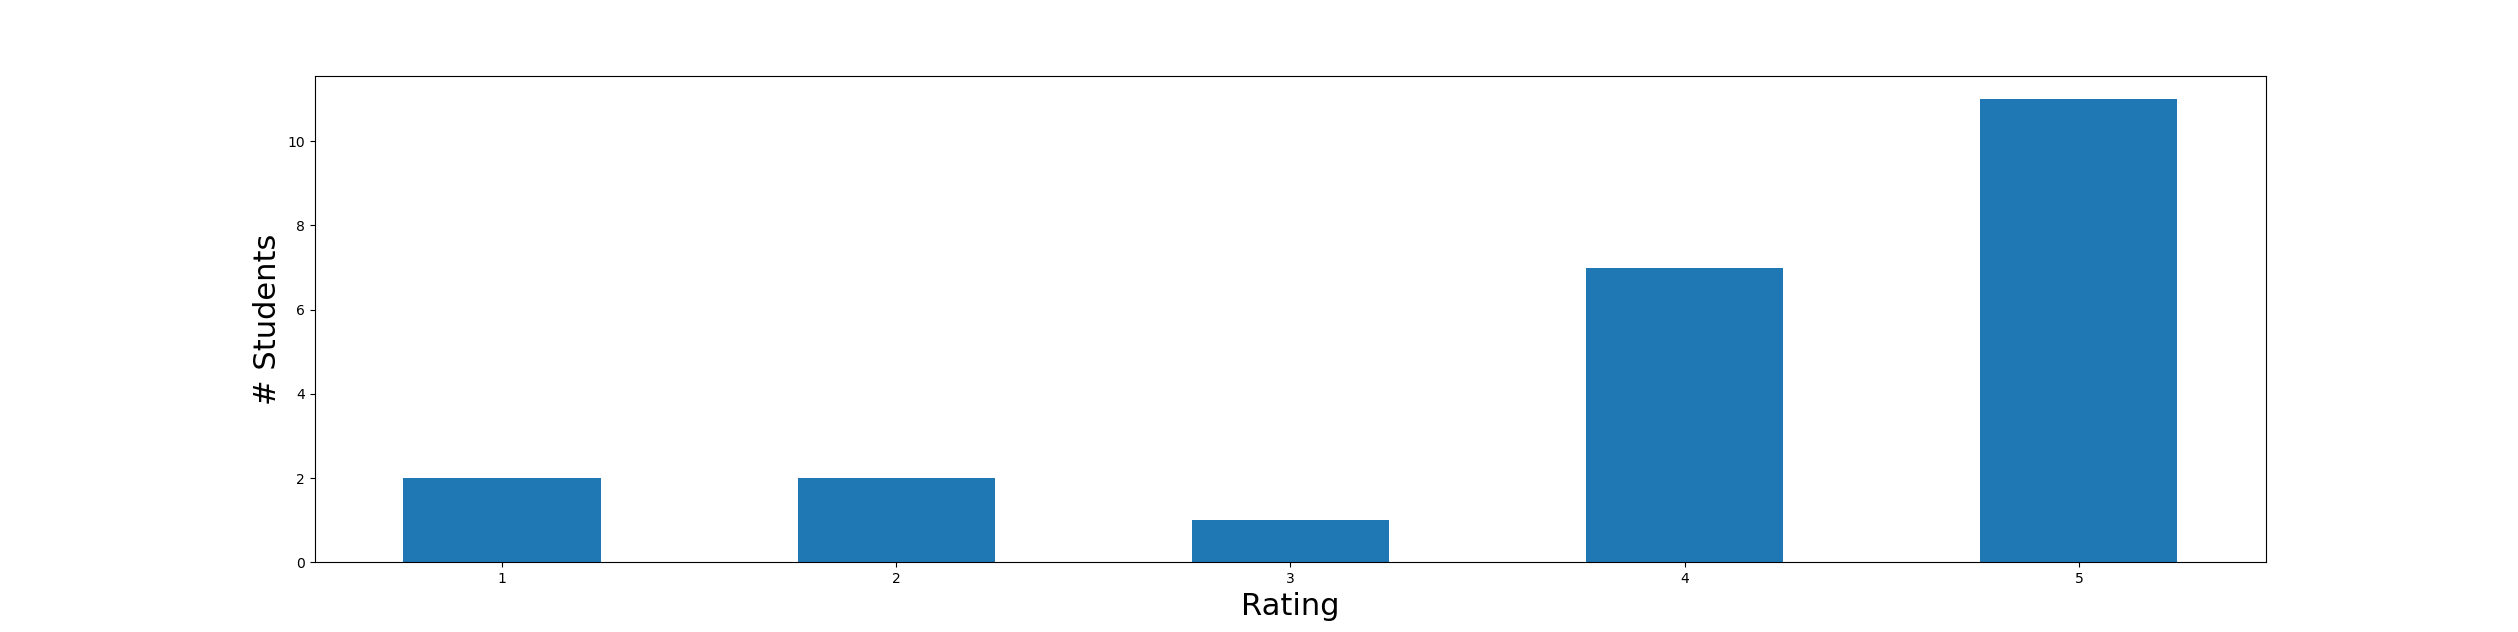
\includegraphics[width=1.0\textwidth,height=0.5\textwidth]{./course-evals/Eval_1XA3_2019_Response.png}
\end{center}

CS 1XA3 was the first time I developed a course completely on my own. I was
employed as a sessional instructor and given full control of what content to
teach, and choose to develop a fully original curriculum. The curriculum was
ambitious, covering a full stack development (Javascript - Python - Django -
MySQL) range of skills in a first year computer science program. I found
myself particularly proud of the amount of independent critical judgement I
encouraged, as was reflected in my course evaluations.

Not all students found my approach effective though. It would be convenient
for me to hand-wave these criticisms as students who weren't ambitious enough
to be in a program as difficult as Computer Science at McMaster. However it's
evident that some of the same students that gave me a low overall
effectiveness still recognized that the class was good for encouraging
independent critical judgement. Being critical of myself, part of the problem
was my lack of flexibility and demeanor when dealing with students who
struggle to initially grasp concepts more than the average student. In later
sessional positions I've taught (such as CS 1JC3), I've continued to try
improve how I approach challenging students without discouraging them.

See the full evaluations for CS 1XA3 2019 C01 at \hyperref[sec:1xa3c01evals]{Appendix C} and C02 at \hyperref[sec:1xa3c02evals]{Appendix C}

\newpage
\subsection{CS 1JC3 C02 Fall 2019}
\label{sec:orgda422f0}

\textbf{Overall for this course, what is your opinion of the effectiveness of the
instructor?} (Scale: 1 Very Poor to 10 Excellent)

\begin{center}
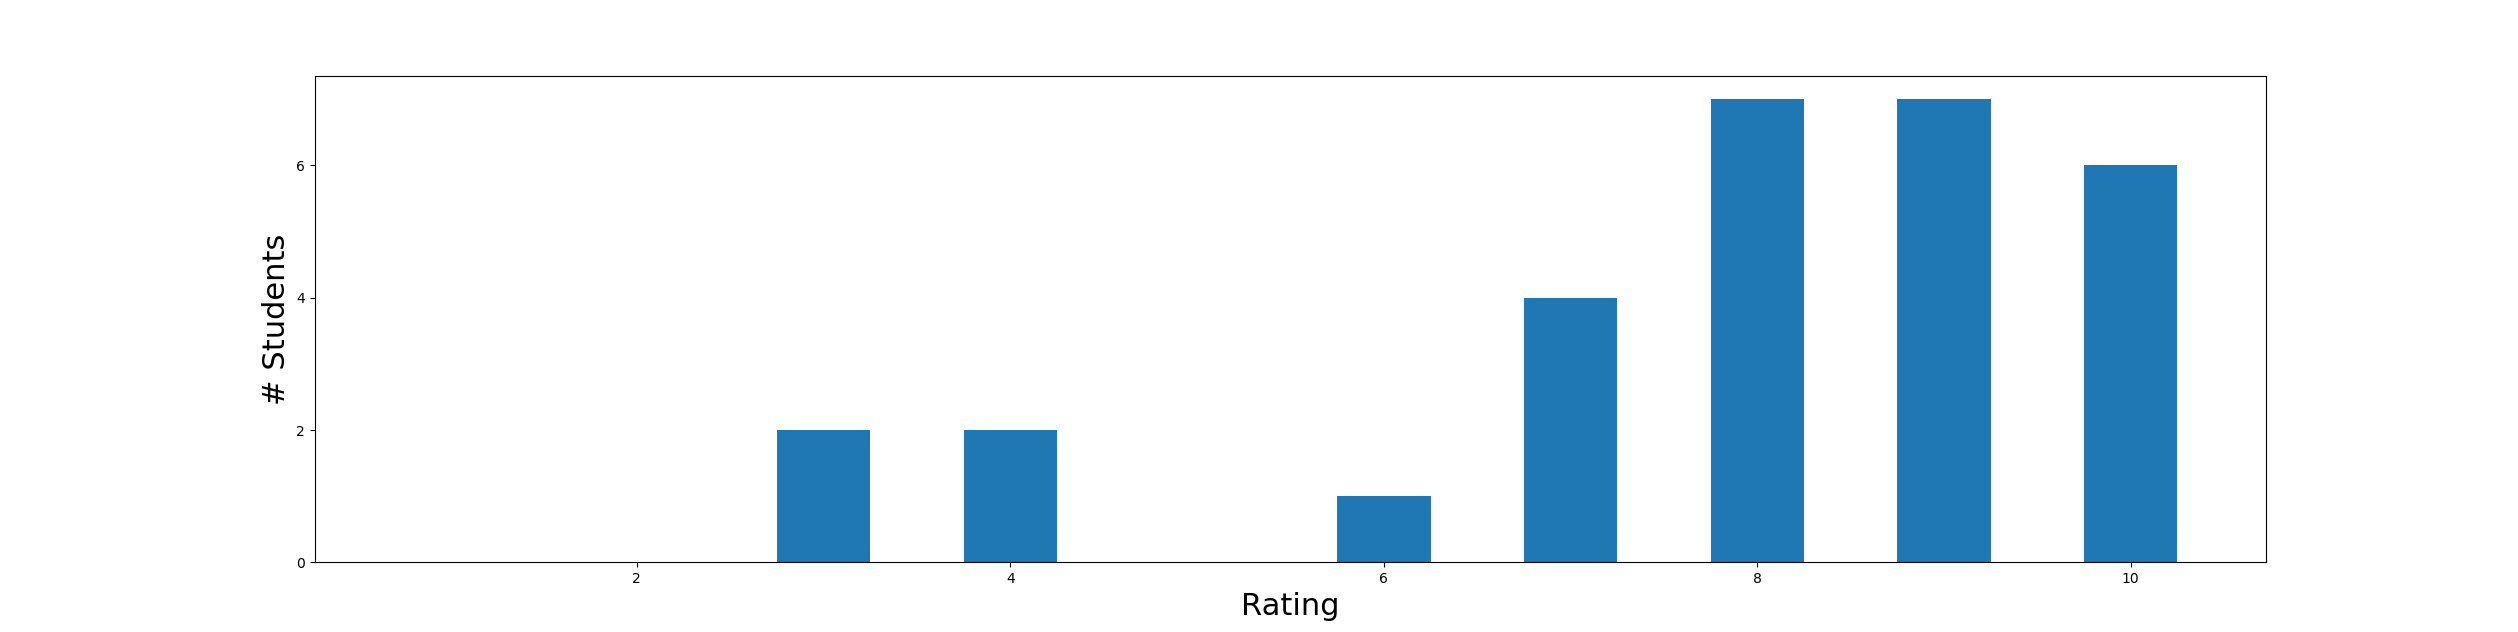
\includegraphics[width=1.0\textwidth,height=0.5\textwidth]{./course-evals/Eval_1JC3_2019_Overall.png}
\end{center}

\noindent
\textbf{Independent critical judgement was encouraged} (Scale: 1 Very Poor to 5 Excellent)

\begin{center}
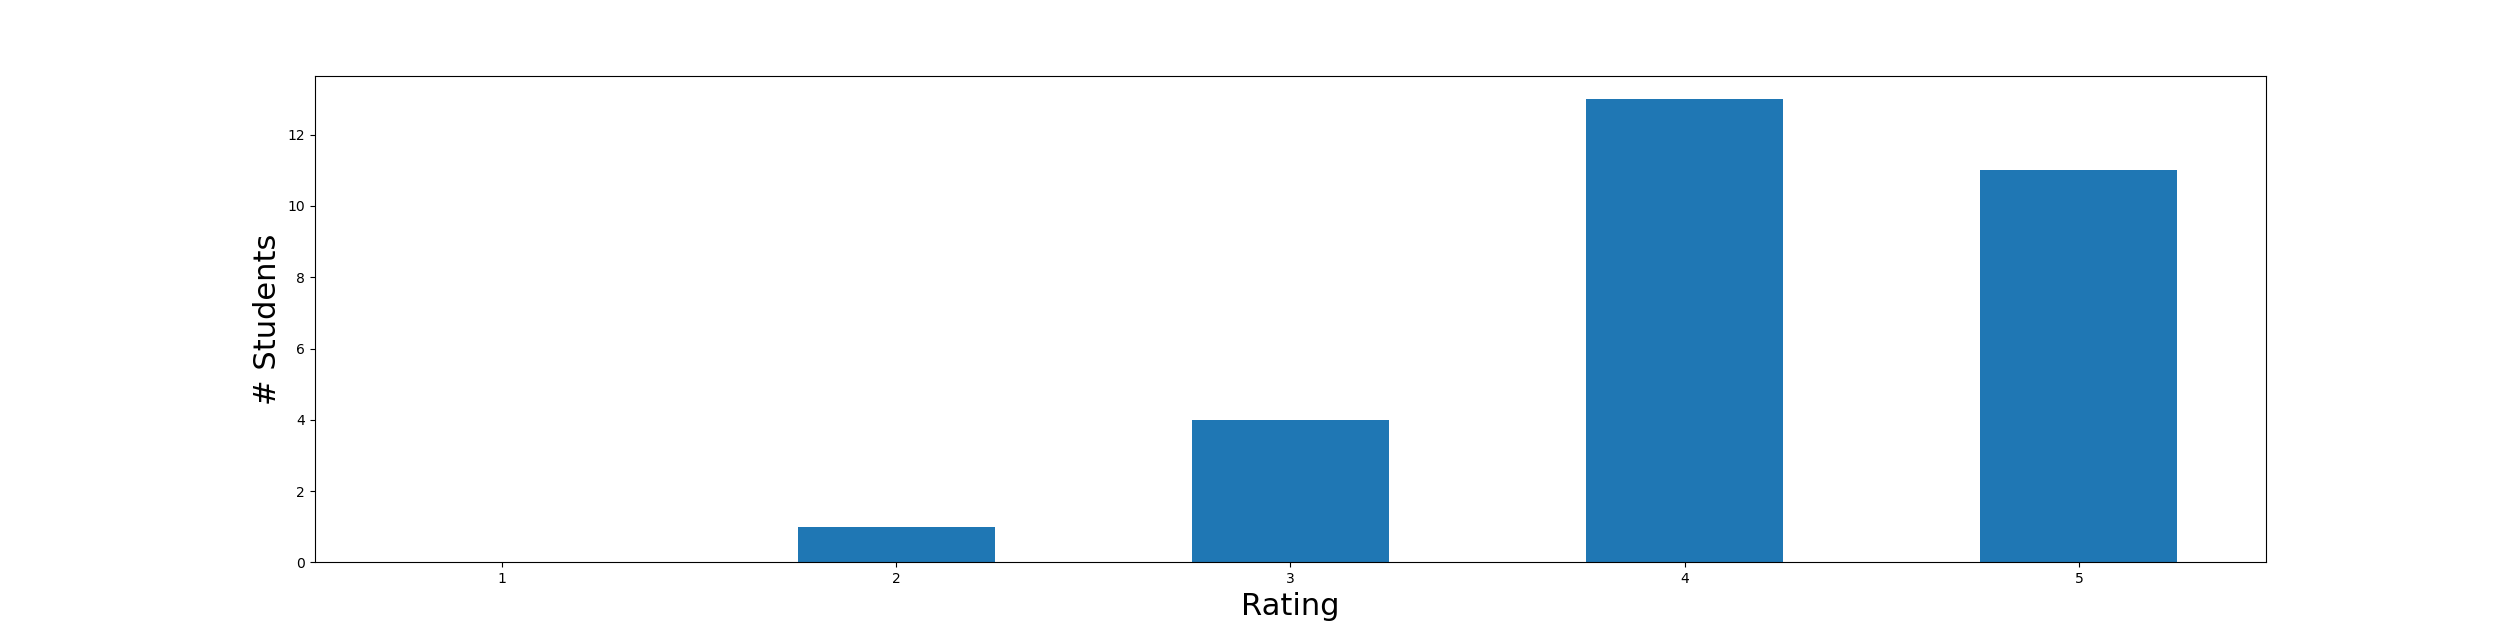
\includegraphics[width=1.0\textwidth,height=0.5\textwidth]{./course-evals/Eval_1JC3_2019_Critical.png}
\end{center}

\newpage
\noindent
\textbf{The instructor's response to students (Approachability, attitude,
availability, well-explained answers)} (Scale: 1 Very Poor to 5 Excellent)

\begin{center}
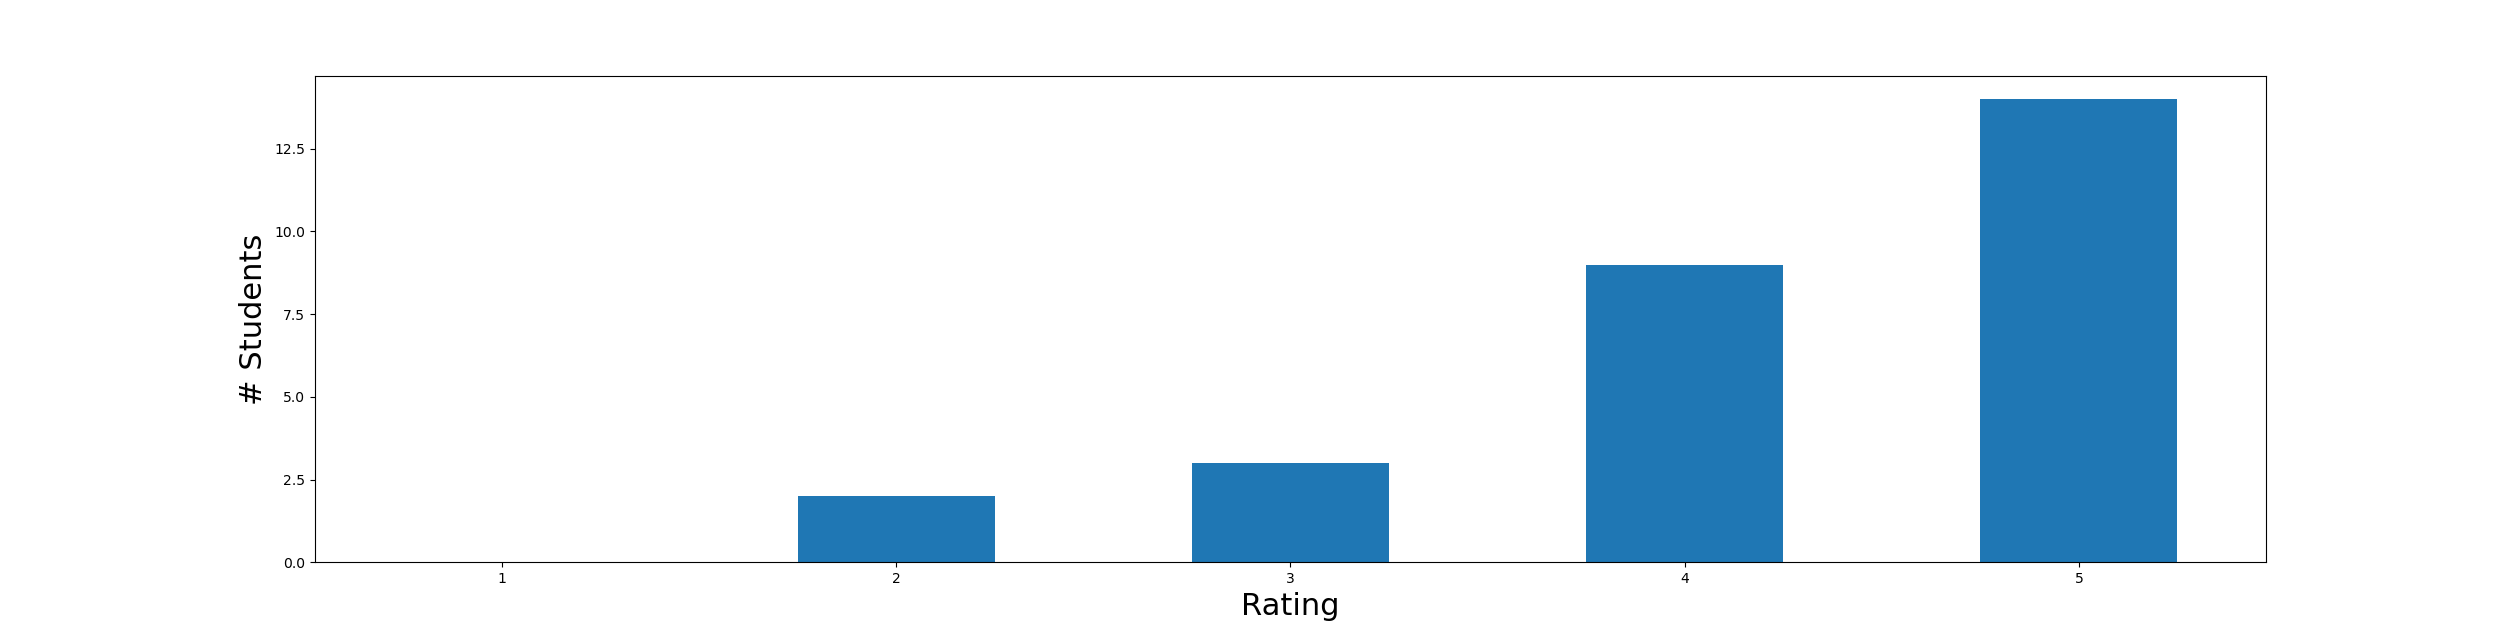
\includegraphics[width=1.0\textwidth,height=0.5\textwidth]{./course-evals/Eval_1JC3_2019_Response.png}
\end{center}

After my winter 2019 session teaching CS 1XA3, I taught CS 1JC3 C02 as a
sessional instructor (alongside another professor who taught CS 1JC3 C01).
The course was split up into two courses, C01 being students enrolled in the
Computer Science program at McMaster, and C02 for students outside the
program (this was done due to the high demand of students wishing to
take an intro programming course). 

Despite being an introductory Computer Science course, CS 1JC3 was a
challenging course covering a wide variety of concepts in computer science
and functional programming. McMaster has high expectations of students
enrolled in Computer Science, and I was tasked with teaching the same content
to students outside of the program for whom computer programming was not
their forte. I did my best to continue to challenge students the way I did in
CS 1XA3, but be more flexible and approachable. Although I still have room to
improve in this respect, by year end it seems less students found me
unapproachable than in CS 1XA3 while still recognizing I valued independent
critical judgement.

See the full evaluations for CS 1JC3 2019 C02 at \hyperref[sec:1jc3evals]{Appendix E}

\newpage
\section{Observations of Teaching}
\label{sec:orgb71b249}
Below are a selection of comments provided by the instructors I have worked
with
\subsection{Dr. Christopher Anand, McMaster Outreach, Supervisor}
\label{sec:orgcee7aa4}
Dr. Anand was my Ph.D supervisor and organizer of McMaster Outreach. In the
future I will include a statement from him about my work with outreach
\subsection{Dr. William Farmer, CS 1JC3 C01 Fall 2019, Instructor}
\label{sec:org6d95bca}
I taught CS 1JC3 alongside Dr. Farmer, in the future I will include a
statement from him 

\part{Teaching Development}
\label{sec:orgeff52e9}
\section{Programs and Certificates}
\label{sec:org20c1eff}
\subsection{MacPherson Institute EDUCATN 750/751}
\label{sec:org29289b1}
\begin{itemize}
\item A graduate course offered by the MacPherson Institute at McMaster University. The
focus is on honing essential pedagogical and practical teaching skills. This
includes sessions on curriculum design, teaching strategies, assessment
strategies, and developing a teaching portfolio.
\item Completed in Winter Semester 2021
\end{itemize}

\section{Conferences}
\label{sec:orgd95c756}
\subsection{Trends in Functional Programming in Education (2017)}
\label{sec:orgec62704}
\begin{itemize}
\item Attendant and presenter at TFPIE 2017 (held at Kent University)
\item The goal of TFPIE is to gather researchers, teachers and professionals
that use, or are interested in the use of, functional programming in
education. TFPIE aims to be a venue where novel ideas, classroom-tested
ideas and work-in-progress on the use of functional programming in
education are discussed.
\end{itemize}

\section{Papers}
\label{sec:org1e632c1}
\subsection{Co-Author: Using Elm to Introduce Algebraic Thinking to K-8 Students}
\label{sec:org4a5f0c2}
\begin{itemize}
\item Research paper analyzing the use of functional programming to teach K-8
students topics in mathematics
\item Published in EPTCS volume 270 \url{http://eptcs.web.cse.unsw.edu.au/paper.cgi?TFPIE2017.2}
\end{itemize}

\part{Future Goals}
\label{sec:orgf3057ca}
\section{Short-Term Goals}
\label{sec:orga6f4624}
In the immediate future, my goals for teaching include:
\begin{itemize}
\item Finish the rest of the MacPherson Institute courses and earn their
Teaching \& Learning Certificates of Completion Program
\item Publish another conference paper on the use of computer science in education
\item Teach CS 1JC3 during the Spring/Summer 2021 session (already underway)
\end{itemize}
\section{Long-Term Goals}
\label{sec:orgf6db81d}

In the next few years, my goals for teaching include:
\begin{itemize}
\item Continue teaching sessional positions as a post-graduate fellow
\item Apply for (and eventually get hired) teaching track (or possibly tenure
track) positions at Colleges/Universities
\end{itemize}

\part{Appendix}
\label{sec:orgc638041}
\appendix
\section{Appendix A: Sample Course Syllabus}
\label{sec:orgb9daa55}
 \label{sec:syllabus}
The following document (see next page) is a sample course syllabus I originally
developed for use in a first year computer science course (CS 1XA3) I taught
as a sessional instructor in 2018/2019 and have since refined

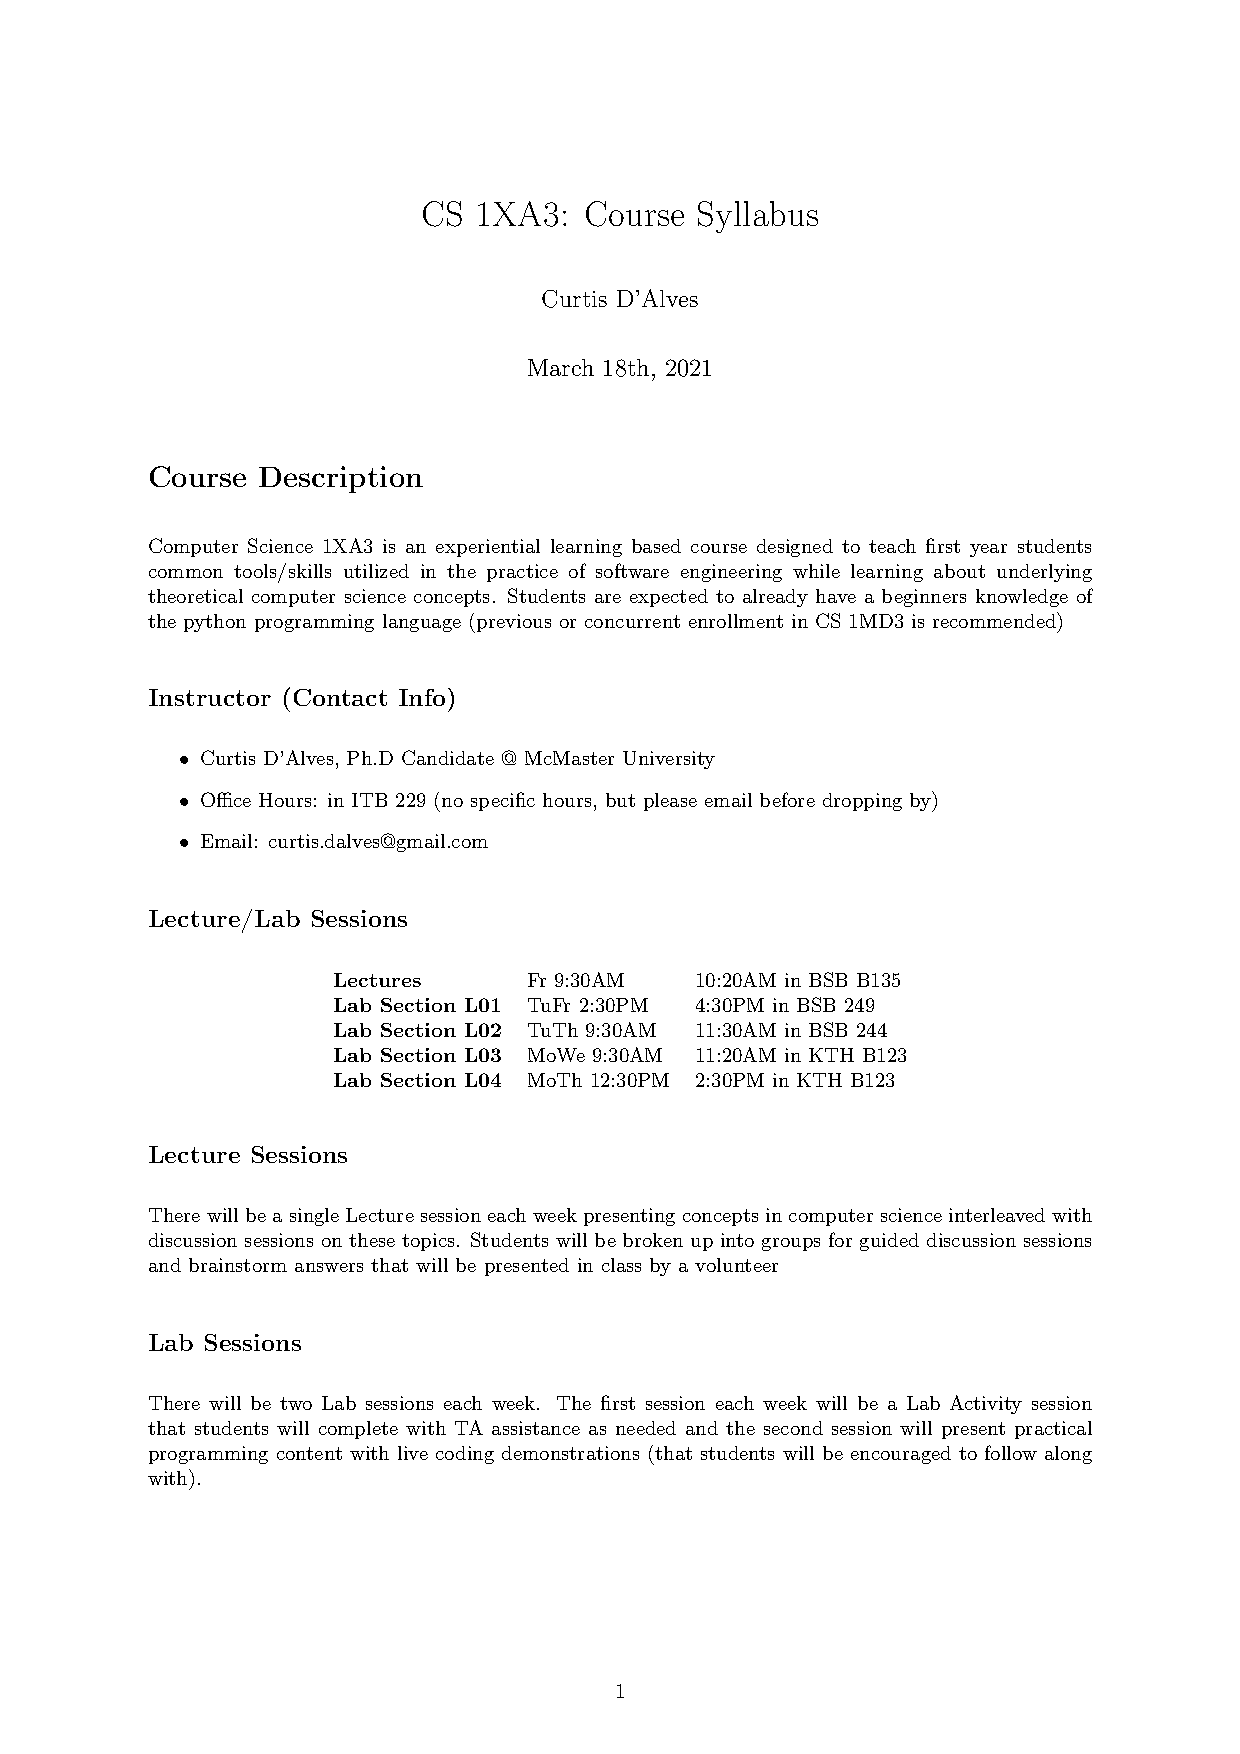
\includepdf[pages=-]{../course-syllabus/Course-Syllabus.pdf}

\section{Appendix B: Sample Assessment}
\label{sec:org2061746}
 \label{sec:assessment}
The following document (see next page) is a sample project I originally
developed for use in a first year computer science course (CS 1XA3) I taught
as a sessional instructor in 2018/2019 and have since refined

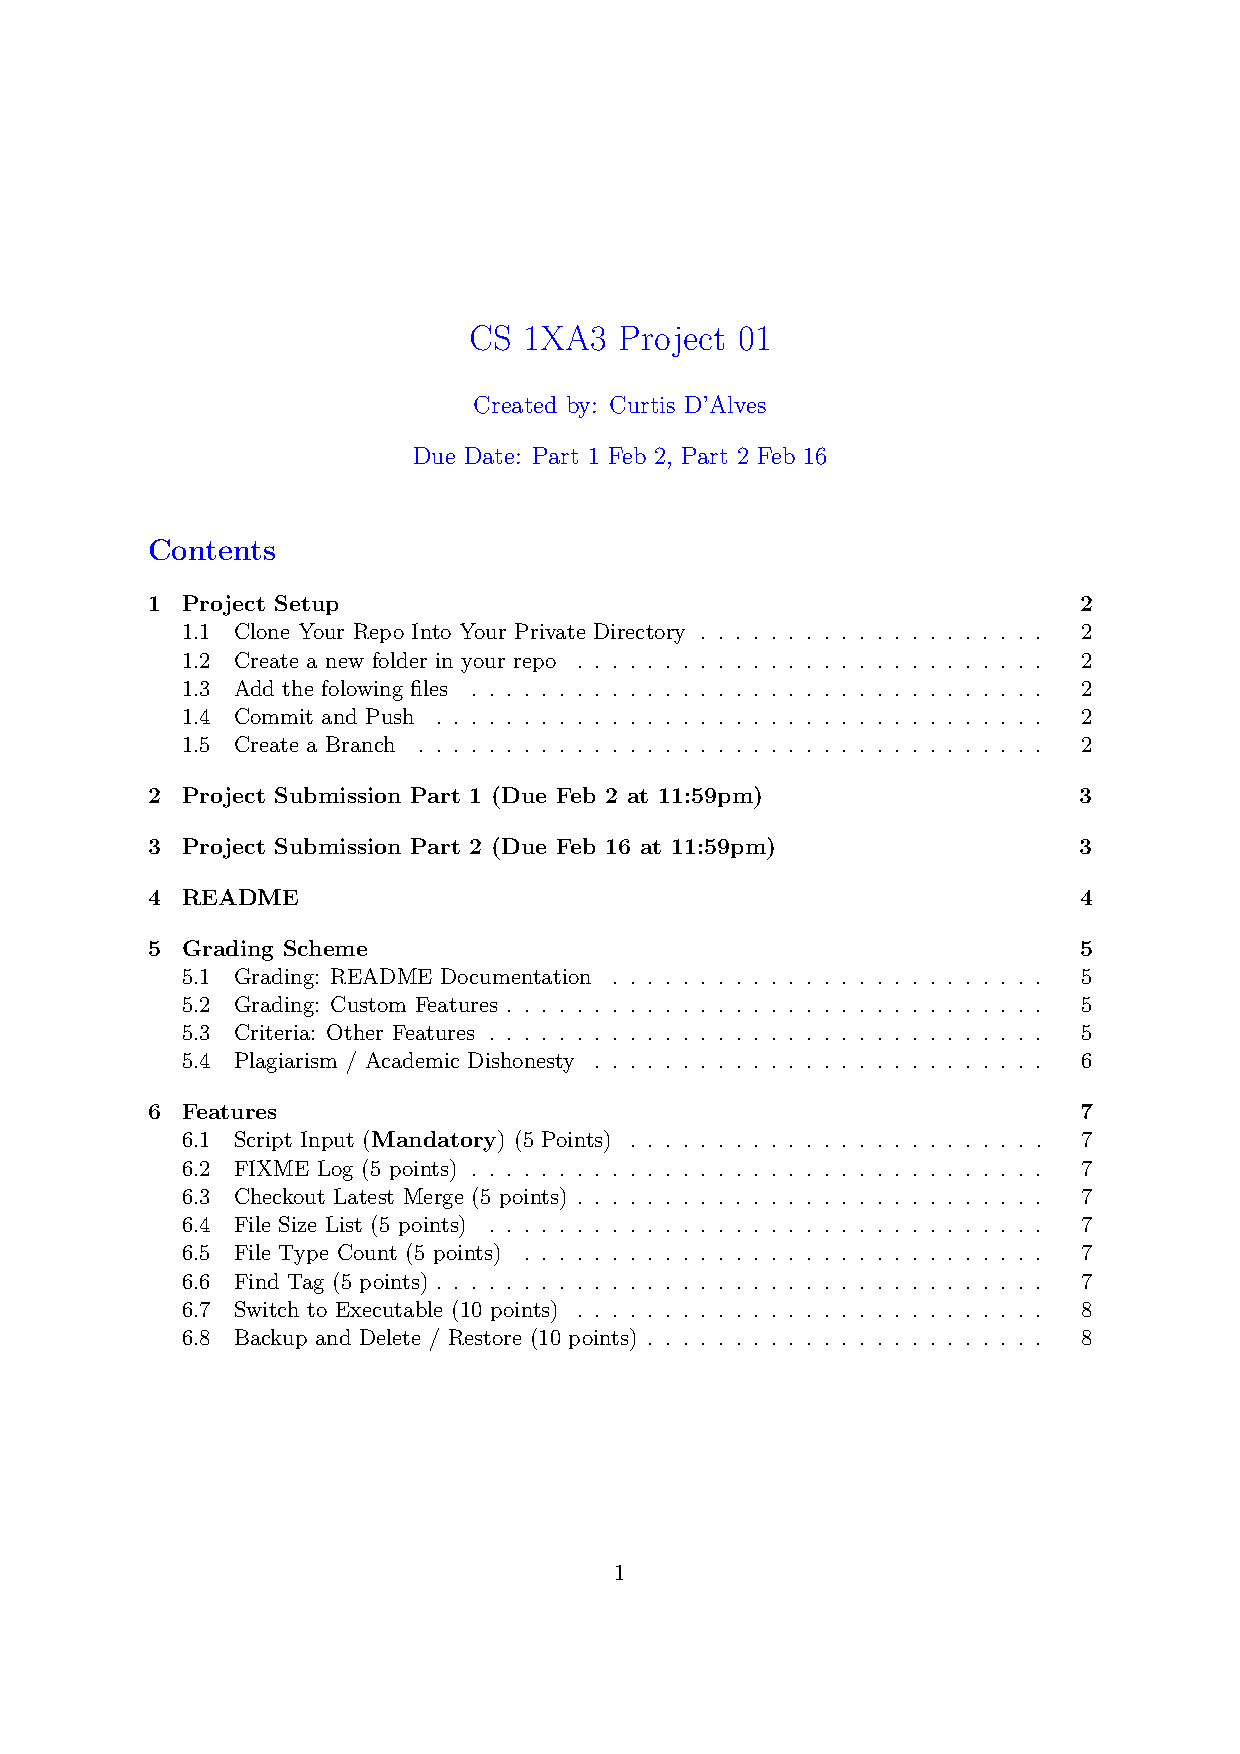
\includepdf[pages=-]{../sample-assessment/Project01.pdf}

\section{Appendix C: Course Evaluation CS 1XA3 2019 C01}
\label{sec:org5e72588}
 \label{sec:1xa3c01evals}
The following document is the course evaluations for CS 1XA3 Winter 2019 section C01
(students enrolled in the Computer Science program at McMaster University). I
taught this section alongside section C02, whose evaluations are in the
proceeding appendix

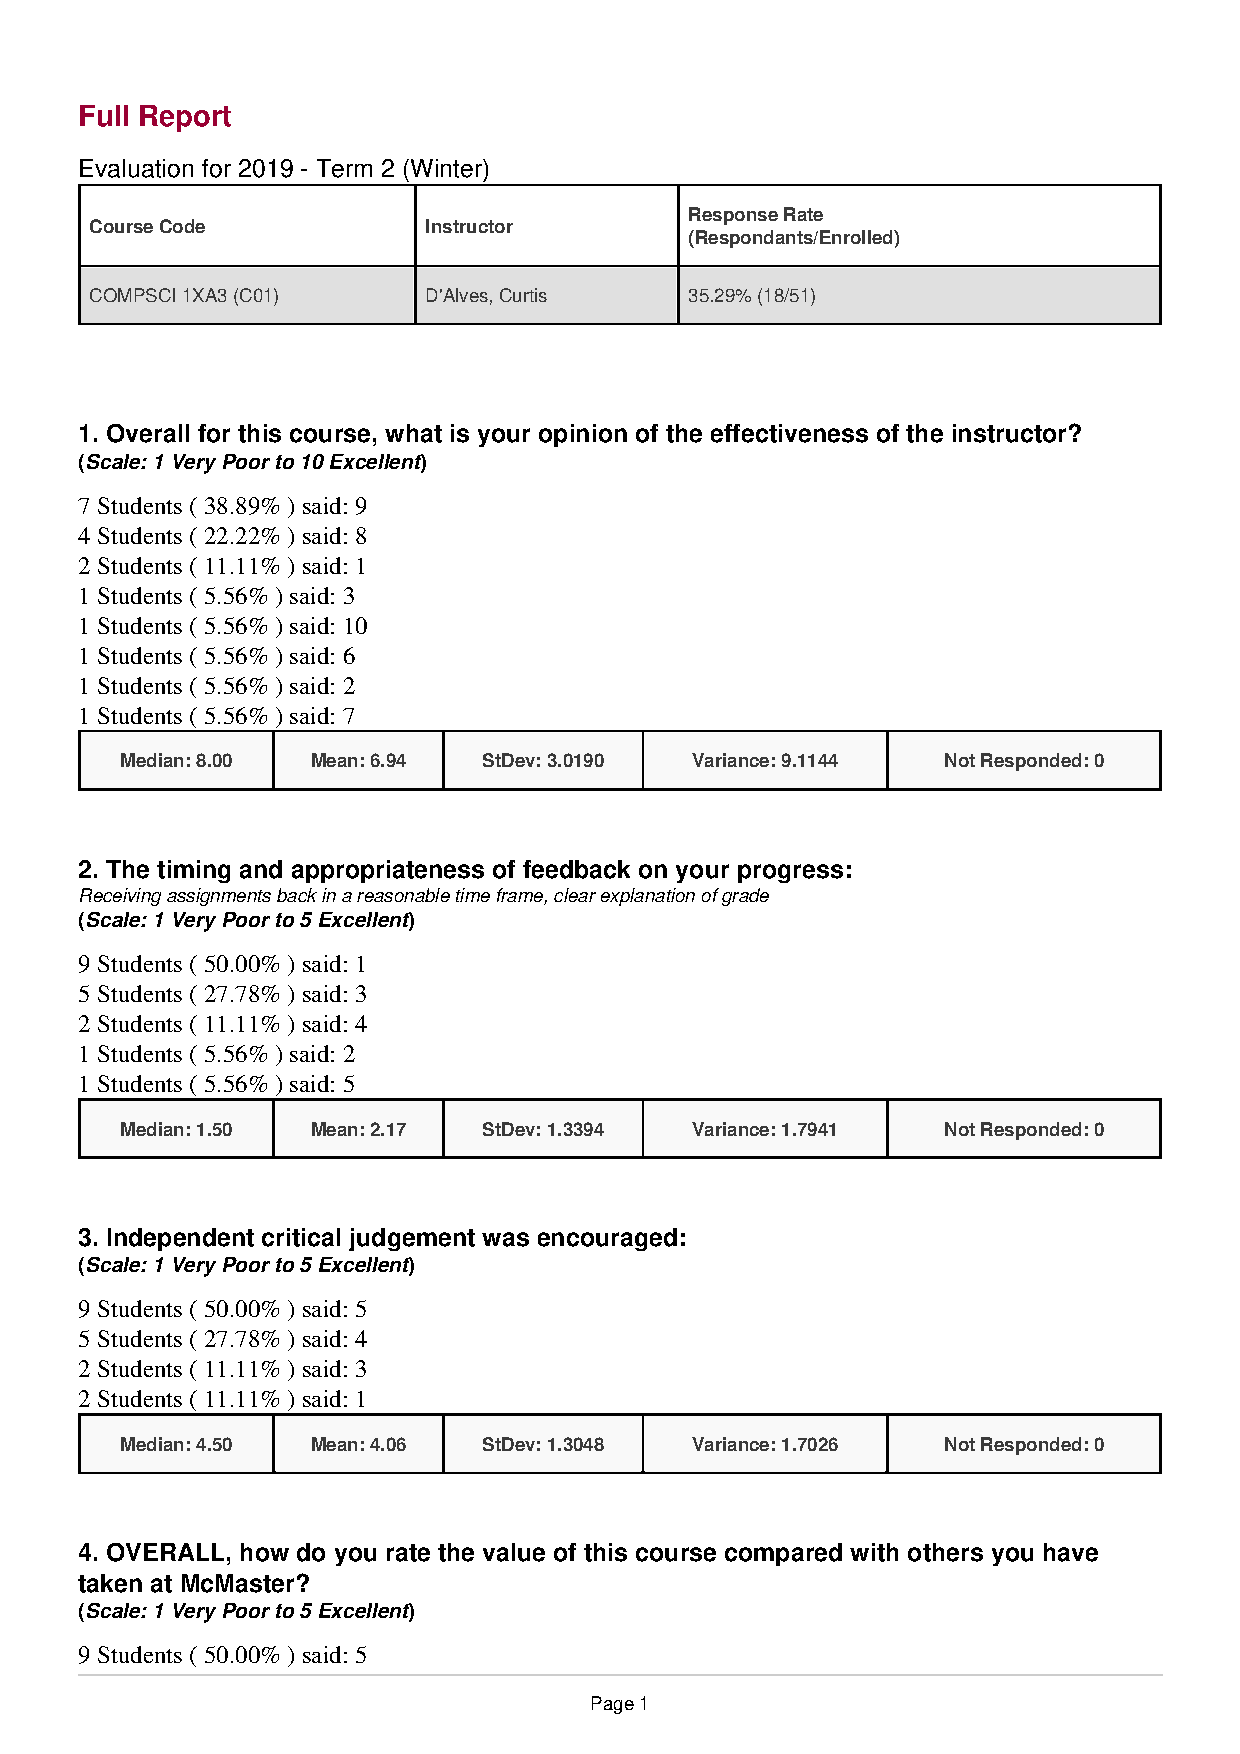
\includepdf[pages=-]{./course-evals/Eval_2019_COMPSCI_1XA3_C01.pdf}

\section{Appendix D: Course Evaluation CS 1XA3 2019 C02}
\label{sec:org92f5d19}
 \label{sec:1xa3c02evals}
The following document is the course evaluations for CS 1XA3 Winter section C02
(students NOT enrolled in the Computer Science program at McMaster University). I
taught this section alongside section C01, whose evaluations are in the
previous appendix

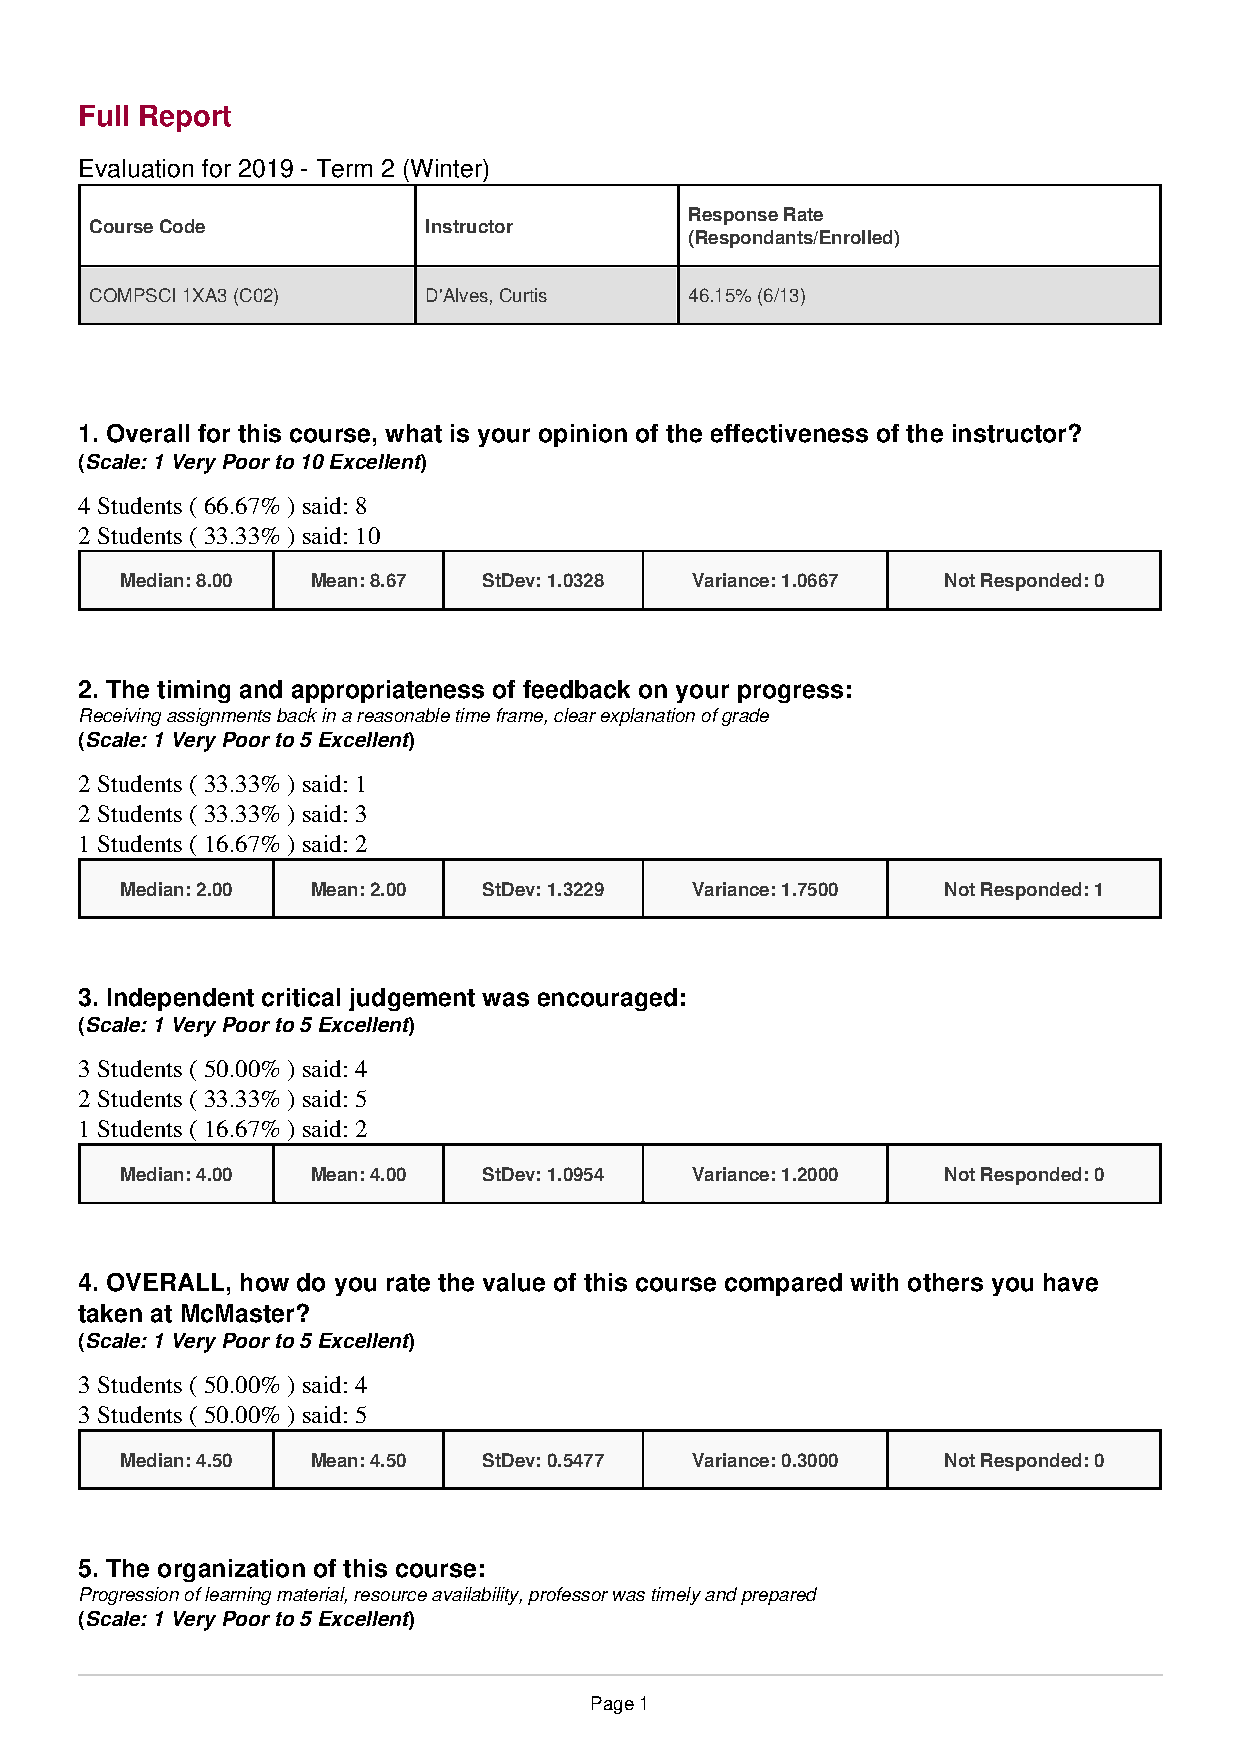
\includepdf[pages=-]{./course-evals/Eval_2019_COMPSCI_1XA3_C02.pdf}

\section{Appendix E: Course Evaluation CS 1JC3 2019 C02}
\label{sec:org80020d4}
 \label{sec:1jc3evals}
The following document is the course evaluations for CS 1JC3 Fall 2019 C02.
(students NOT enrolled in the Computer Science program at McMaster University). I
taught this section separate from section C01, which was taught by Dr. William Farmer  

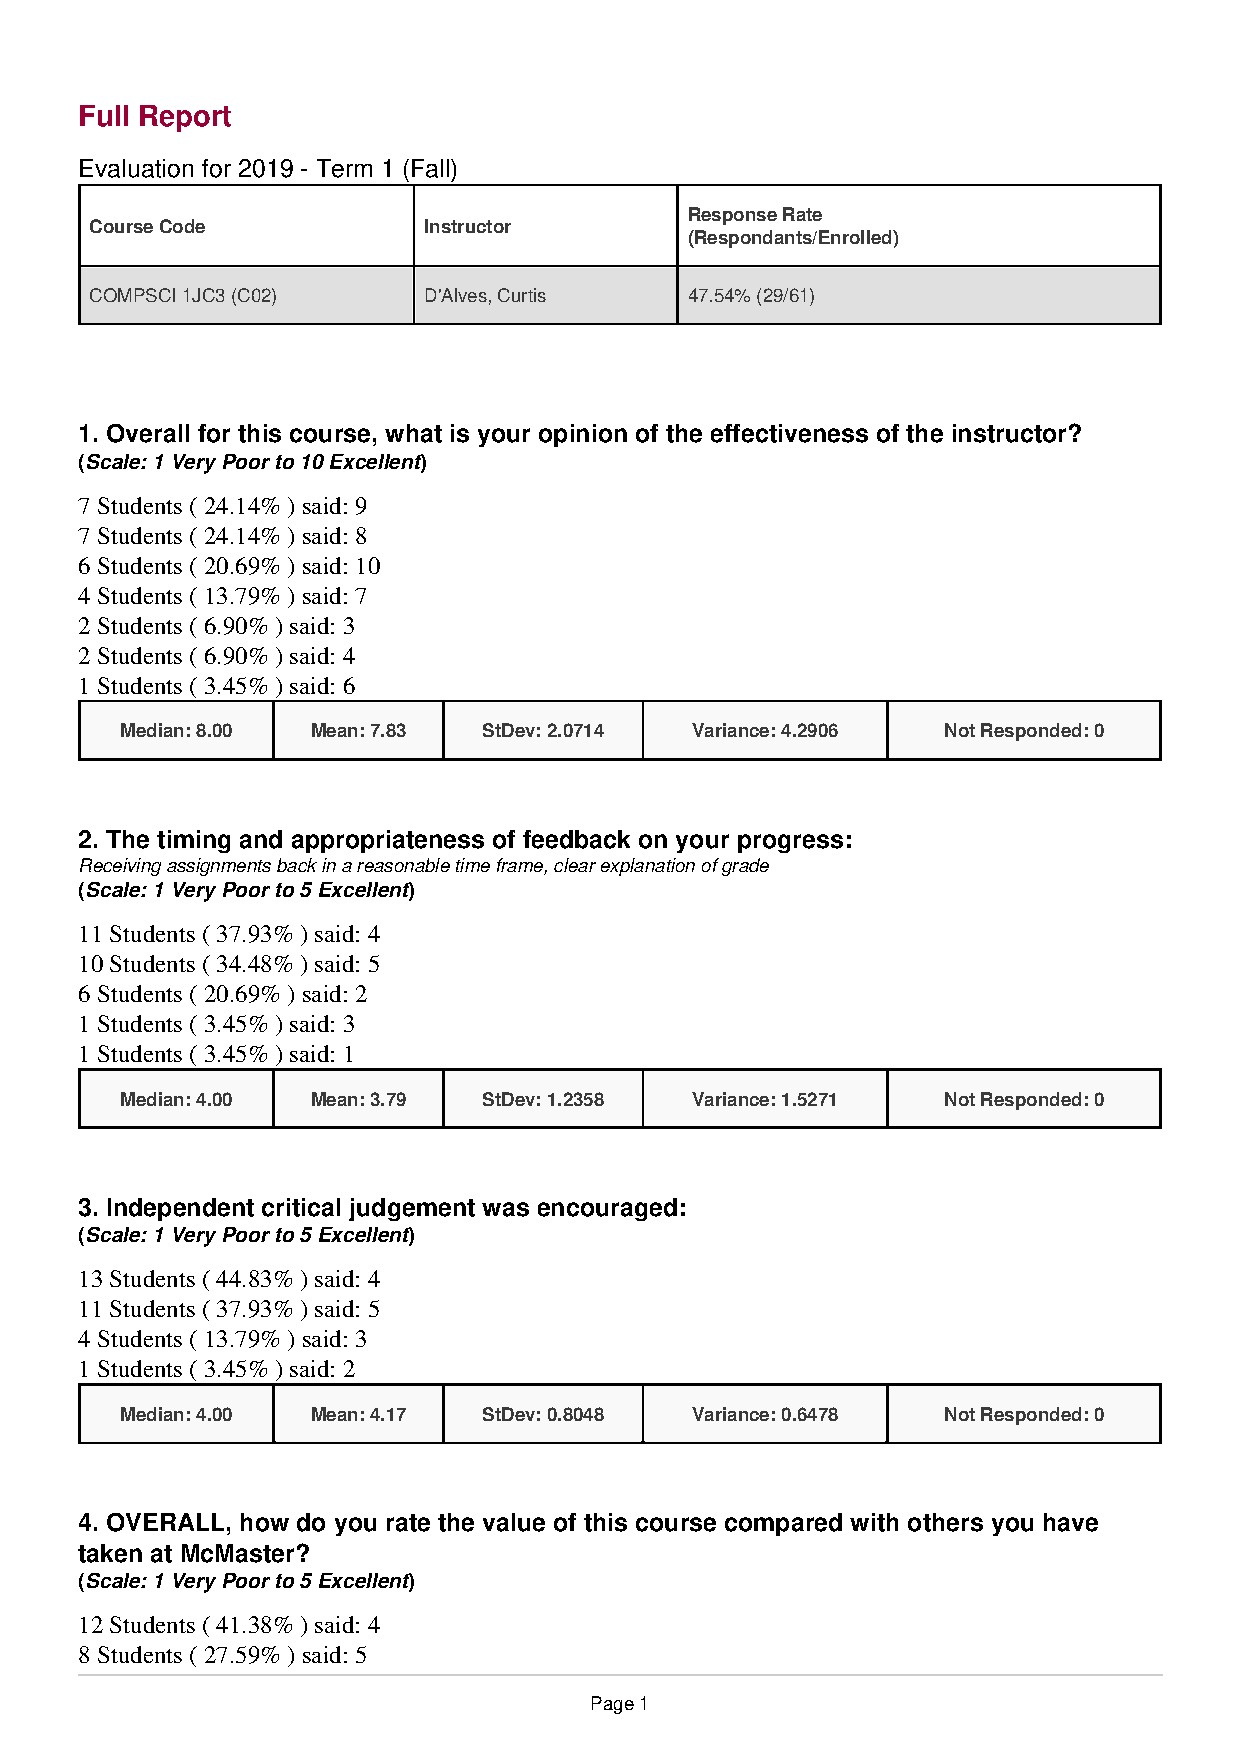
\includepdf[pages=-]{./course-evals/Eval_2019_COMPSCI_1JC3.pdf}
\end{document}